\documentclass{article}
\usepackage[utf8]{inputenc}
\usepackage{graphicx}
\usepackage{geometry}
\usepackage{hyperref}
\usepackage{float}
\usepackage{titlesec}

\setcounter{secnumdepth}{4}

\titleformat{\paragraph}
{\normalfont\normalsize\bfseries}{\theparagraph}{1em}{}
\titlespacing*{\paragraph}
{0pt}{3.25ex plus 1ex minus .2ex}{1.5ex plus .2ex}

\hypersetup{
    colorlinks,
    citecolor=black,
    filecolor=black,
    linkcolor=black,
    urlcolor=black
}

 \geometry{
 a4paper,
 left=30mm,
 right=30mm,
 top=30mm,
 }

\graphicspath{ {./../Images/} }

%----------------------------------------------------------------------------------------
%	TITLE PAGE
%----------------------------------------------------------------------------------------

\newcommand*{\titleGP}{\begingroup
		\begin{figure}[t]
			\centering
			
\includegraphics[width=350px]{UP_Logo.png}
		\end{figure}
\centering

{\Large COS 301 Capstone Project 2017}

\vspace*{\baselineskip}

\rule{\textwidth}{1.6pt}\vspace*{-\baselineskip}\vspace*{2pt}
\rule{\textwidth}{0.4pt}\\[\baselineskip]

{\Huge Vulknut Software Engineering } \\ [0.2\baselineskip]

\rule{\textwidth}{0.4pt}\vspace*{-\baselineskip}\vspace*{2pt}
\rule{\textwidth}{0.4pt}\\[\baselineskip]

{\Large SRS Documentation } \\ [0.2\baselineskip]

\rule{\textwidth}{0.4pt}\vspace*{-\baselineskip}\vspace{3.2pt}
\rule{\textwidth}{1.6pt}\\[\baselineskip] %

% \scshape %
% A concise specification on the functional requirements  \\
% and use cases of NavUP \\[\baselineskip]

% \vspace*{2\baselineskip}

\bigskip

Compiled By \\[\baselineskip]

\bigskip

{\Large Peter Boxall - u14056136 \\ Claude Greeff - u13153740 \\ Marin Peroski -  u13242475 \\ Johan du Plooy - u12070794 \\ Bernhard Schuld - u10297902 \\\par}

\bigskip
\bigskip

	\begin{figure}[H]
			\centering
			
\includegraphics[width=200px,height=125px]{epiUse.png}
	\end{figure}

\bigskip
\bigskip

 {\Huge 3D VR Presentations}

\vfill

 	{\large GitHub Repository:
 	\href{https://github.com/Valknut-Software-Engineering/Capstone_Project}{Valknut Software Engineering}\par}

\endgroup}


\begin{document}

\titleGP
\newpage
\tableofcontents
\newpage


\section{System Requirements and Design}

\subsection{Introduction}

	\subsubsection{Purpose}
	This document serves to outline the overall description and requirements of 	the system. This document also serves as a guideline to the developers in 		order to ensure the final product meets these requirements, and indicates 		to the client what the required technologies are in order to be able to use 	this system.

	\subsubsection{Scope}

	The overall objective of this project is to provide any given user with a toolkit, with which the individual can create a 3D virtual reality presentation with ease. Our goal is to make it simple to use, enabling virtually any user to utilize the power of 3D, without having to build 3D objects completely from scratch. The user would custom build a 3D environment built upon a variety of available templates offered, or by selecting a set of 3D models and skyboxes when choosing to create a project from the ground up, taking user experience to a whole nother level.

	\subsubsection{Definitions, Acronyms and Abbreviations}
			\paragraph{VR}	Virtual Reality
			\paragraph{MVP} Minimum Viable Product
			\paragraph{MTBF} Mean Time Between Failures
			\paragraph{e2e} End-To-End


		% \section{References}

	\subsubsection{Software Description}

	Presentation software such as Microsoft's Power Point, have been around for almost 2 decades now.  However due to many constraints and limited hardware capabilities, these presentations are only available as a 2D representation. With Virtual and Augmented reality growing ever more popular and easily accessible, should it not be possible to add a 3rd dimension to our presentations? This software aims to do exactly that. \\

	This software will make it possible for virtually anyone familiar with a computer to design and edit 3D presentations, to be viewed via the use of VR headsets such as the HTC VIVE and the Oculus Rift. After selecting to create a new project for example, a user would be presented with a 3D world that will be mostly empty at first.  The user can then select from a variety of customization options and toolboxes to modify and add content to their world. \\

	When the user is satisfied with the world they see before them, they can then create a method of presentation, such as recording a tour through the world, that can even feature their voice if the user so desires.  At any point during presentation recording, the user can still modify any part of their surrounding world, if for example they change their mind about the placement of an object, or even the lighting in a room to name but a few.

	Finally when the user has finished setting up the entire presentation, they can choose to export the final product as a 360 degree video, that can then be viewed on any device that supports 360 videos.  Then at the time of presentation, everyone in the audience will be able to join in so long as they have a VR headset at their disposal.

\subsection{Design}

	\subsubsection{Software Methodology}
	We will follow the Agile development methodology. The principles this methodology is based on advocates planning, constantly evolving development, early delivery and continuous improvements. It encourages flexibility as well as maintainability.

	\begin{flushleft}
	The agile development process is built on four main principles:
		\begin{enumerate}
			\item Individual and team interactions over processes and tools.
			\item Working software over comprehensive documentation.
			\item Customer collaboration over contract negotiation.
			\item Responding to change over following a plan.
		\end{enumerate}
	\end{flushleft}

	\begin{flushleft}

	The Agile development approach allows for frequent opportunities for clients to be involved in. Requirements are then re-prioritized according to client specifications and they are elaborated on. The process of Agile development is based on the following actions:

	\end{flushleft}

    \begin{itemize}
			\item Short timeboxes of iterative development.
			\item Early and repeated client/user feedback.
			\item Re-prioritisation of work based on the client/user so that emergent requirements can be handled.
			\item Selecting a specific approach of which there are a variety of options including, Extreme Programming, Scrum, Lean Development, and Feature-Driven Development.
	\end{itemize}

Some of the benefits of using the Agile development include stakeholder engagement, transparency, early and predictable delivery, predictable costs and schedule, allows for change, focus on the client, and ultimately improving the quality of the software. \\

For the above-mentioned reasons, we had chosen to utilize the Agile Software Methodology as it was the most applicable satisfying our needs as well as our client's.

	\subsubsection{Development Technique}
	During our first meeting with EPI-USE they had mentioned that we should make use of a development technique called MVP. A MVP is the most basic version of a product that can still be released. The point of this technique would be that early adopters would see the potential that the final product could offer, and give developers valuable feedback needed to guide them forward.
	
\newpage

\subsection{System Requirements}

The Virtual Reality presentation software will have various requirements that will need to be fulfilled in order to deliver a viable product.

	\subsubsection{Functional Requirements}

	The following functional requirements will be met:

		\paragraph{360 video export}

		The software must be able to export a presentation as a 360 degree video.
		The reason for this exporting format is to allow for a viewable format that will be as universal as possible to all VR capable devices ranging from mobile phones to VR headsets.

		\paragraph{VR Device Viewable}

		The software must be able to be viewable and intractable with the use of a Virtual Reality headset such as the Oculus Rift and HTC Vive.
		A user must be able to preview his or her virtual reality presentation within a virtual reality environment if they own the appropriate hardware as well as edit the environment in virtual reality space.

		\paragraph{Selectable Skyboxes}

		There needs to be a variety of skyboxes that a user can select from in order to match the theme of the environment.
		The skyboxes also need to be compatible with the Unity engine in order to be incorporated into the scene properly.

		\paragraph{Template Environments}

		Template environments must be available to the user.
		These environments will vary to allow for a range of scenes to be catered for.
		A small set of template environments will be created by the development team and the rest by the community (community driven software approach).

		\paragraph{Various Object Imports Into Scene}

		A variety of objects will need to be available for placement in the scene.
		These objects will need to be compatible with the Unity engine as well as relate to some possible environment.
	  Users should be allowed to import their own objects as well as objects created by the community.

		\paragraph{Editor Pont of View}

		The placement and control of the point of view of the user who is currently editing the scene (whether using a VR device or not) is vital.
		The user will need to be able to either walk on the terrain of the environment or be able to fly in the environment for better perspective of the presentation.

		\paragraph{Native Interface Design}

		The interface for the software will need to run in the Windows environment as the application is being developed for the Windows operating system.
		It will also need to be easy to use and navigate.

	\subsubsection{Non-Functional Requirements}

	The following non-functional requirements will be met:

		\paragraph{Image Importing}

		Images the creator wants to display in the scene will need to be able to be imported into it.
		The .jpg image format will be used for the images as it is the most commonly found image format.

		\paragraph{Slideshows}

		Imported images must be able to be incorporated into a slideshow or multiple slideshows.
		These will allow the creator to describe a topic in detail through various images that relate to the subject matter.

		\paragraph{Video Importing}

		Videos allow for a rich and detailed explanation of the topics the user is trying to cover.
		The .ogv video format will be used to incorporate videos into the presentation that can be viewable in the virtual reality space.

		\paragraph{Audio Importing}

		The software will need to be able to incorporate audio snippets or songs into the scene.
		The .ogg audio format will be used for audio files.
		Voice recordings will also fall part of the audio file requirement as they are an important asset that can be incorporated into the presentation.
		This will allow the creator to direct a user's attention to a certain part of the scene.
		It will also allow the creator to describe parts of the presentation to the viewer.
		The software must be able to import voice recordings users make and save with third party applications.

		\paragraph{Community Driven Content}

		The software will need to be able to allow users to create their own content and upload it to a central server which can then be viewed and downloaded by any user who wishes to use the created content.
		This will cover environmental scenes, 3D objects, presentation templates, skyboxes and other Unity based assets that are supported by the software.

\subsection{Application Design}
	\subsubsection{Use Cases}

	\begin{flushleft}
	The following services are provided for the presentation creator.

	\begin{itemize}
		\item Scene Selection:
	\end{itemize}


	\begin{center}
	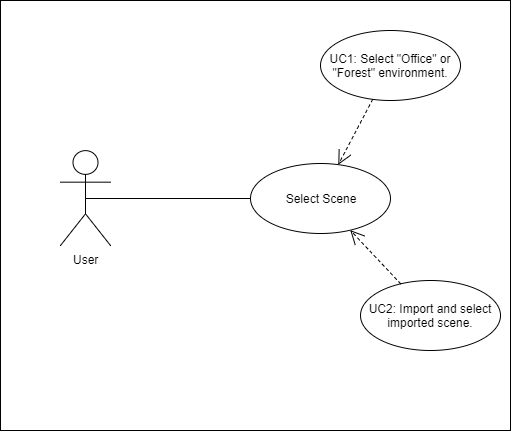
\includegraphics[width=250px,height=150px]{SceneSelection.png}
	\end{center}

	\textbf{Precondition:} The user has the "Office" and "Forest" scene in their asset project folder.

	\textbf{Postcondition:} The user is spawned within the selected environment.

	\newpage

	\begin{itemize}
		\item Object Creation:
	\end{itemize}


	\begin{center}
	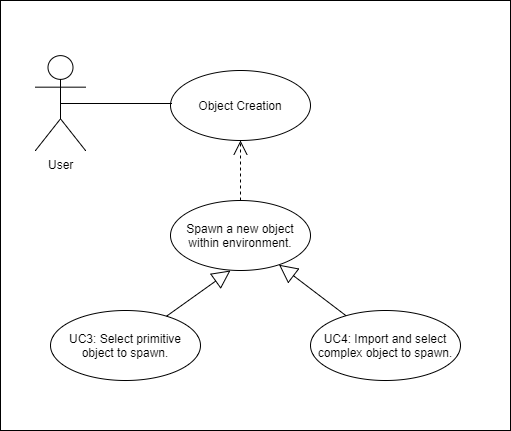
\includegraphics[width=250px,height=150px]{ObjectCreation.png}
	\end{center}

	\textbf{Precondition:} The user is inside an environment.

	\textbf{Postcondition:} The selected object is spawned in front of them.

	\begin{itemize}
		\item Object Cloning:
	\end{itemize}

	\begin{center}
	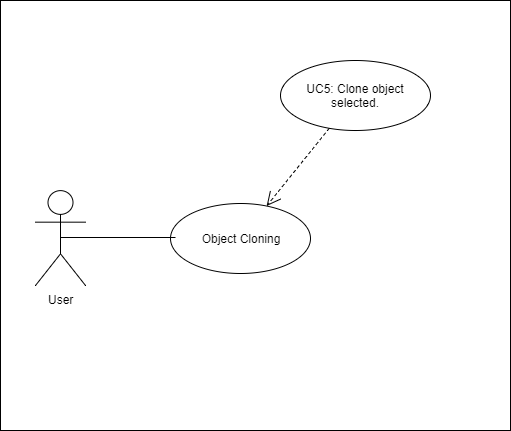
\includegraphics[width=250px,height=150px]{ObjectCloning.png}
	\end{center}

	\textbf{Precondition:} The user selectes the specific object to clone.

	\textbf{Postcondition:} A duplicate of the selected object is spawned.

	\begin{itemize}
		\item Object Deletion:
	\end{itemize}

	\begin{center}
	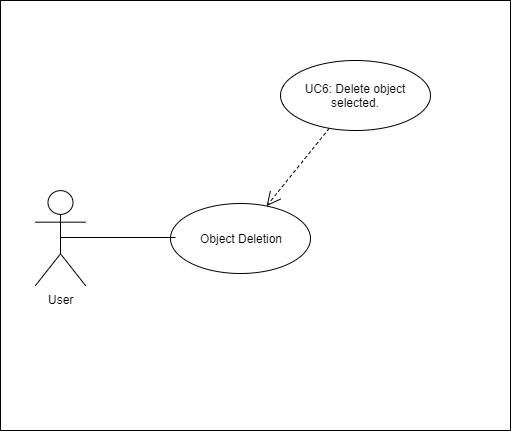
\includegraphics[width=250px,height=150px]{ObjectDeletion.png}
	\end{center}

	\textbf{Precondition:} The user selects the specific object to delete.

	\textbf{Postcondition:} The object is removed from the environment.

	\newpage

	\begin{itemize}
		\item Object Scaling:
	\end{itemize}

	\begin{center}
	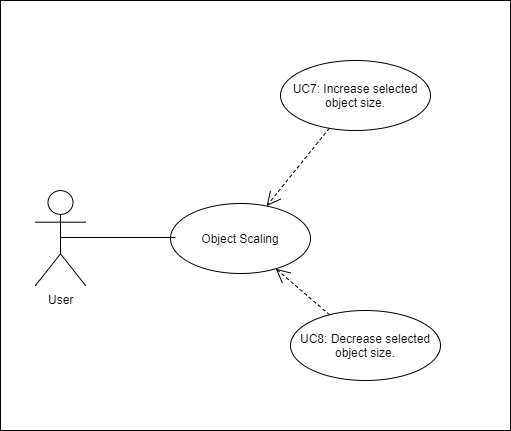
\includegraphics[width=250px,height=150px]{ObjectScaling.png}
	\end{center}

	\textbf{Precondition:} The user selects the specific object to scale.

	\textbf{Postcondition:} The object is scaled up or down.

	\begin{itemize}
		\item Object Interaction:
	\end{itemize}

	\begin{center}
	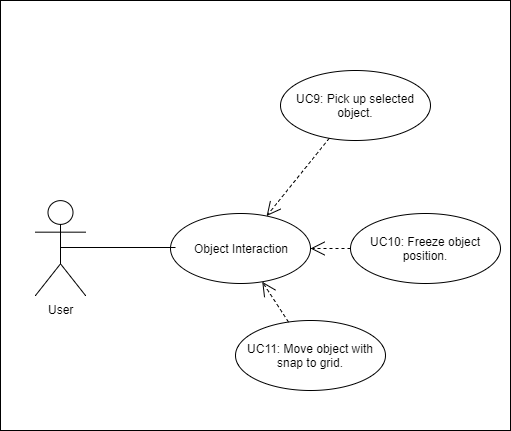
\includegraphics[width=250px,height=150px]{ObjectInteraction.png}
	\end{center}

	\textbf{Precondition:} The user selects the specific object.

	\textbf{Postcondition:} The object is picked up.

	\textbf{Postcondition:} The object is frozen in it's current position.

	\textbf{Postcondition:} The object is moved using the snap to grid movement.

	\begin{itemize}
		\item Object Rotation:
	\end{itemize}

	\begin{center}
	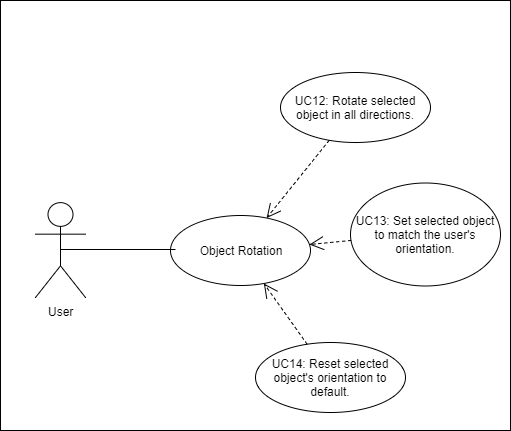
\includegraphics[width=250px,height=150px]{ObjectRotation.png}
	\end{center}

	\textbf{Precondition:} The user selects the specific object.

	\textbf{Postcondition:} The object is rotated accordingly.

	\newpage

	\begin{itemize}
		\item Audio Attachment:
	\end{itemize}

	\begin{center}
	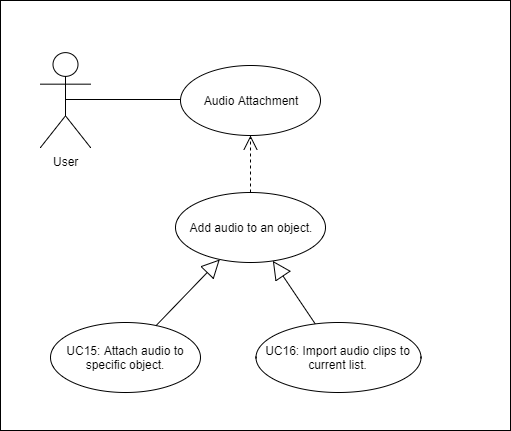
\includegraphics[width=250px,height=150px]{AudioAttachment.png}
	\end{center}

	\textbf{Precondition:} The user selects the specific object to whom the user wishes to attach the audio clip to.

	\textbf{Postcondition:} The audio clip is attached to that specific object.

	\begin{itemize}
		\item Image Attachment:
	\end{itemize}

	\begin{center}
	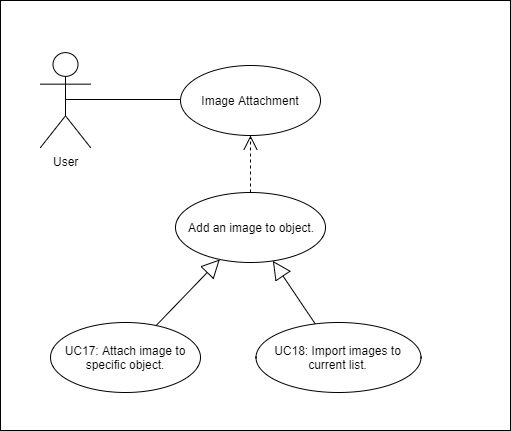
\includegraphics[width=250px,height=150px]{ImageAttachment.png}
	\end{center}

	\textbf{Precondition:} The user selects the specific object to whom the user wishes to attach the image to.

	\textbf{Postcondition:} The image is attached to that specific object.

	\begin{itemize}
		\item Text Attachment:
	\end{itemize}

	\begin{center}
	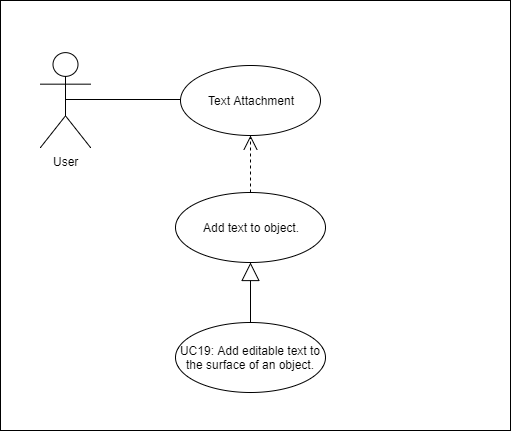
\includegraphics[width=250px,height=150px]{TextAttachment.png}
	\end{center}

	\textbf{Precondition:} The user selects the specific object to whom the user wishes to attach the text to.

	\textbf{Postcondition:} The text is attached to that specific object.

	\begin{itemize}
		\item Video Attachment:
	\end{itemize}

	\begin{center}
	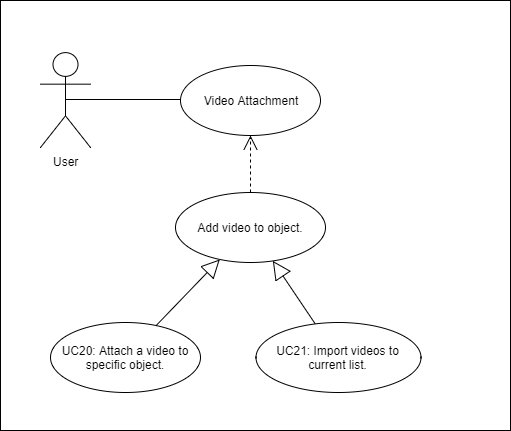
\includegraphics[width=250px,height=150px]{VideoAttachment.png}
	\end{center}

	\textbf{Precondition:} The user selects the specific object to whom the user wishes to attach the text to.

	\textbf{Postcondition:} The text is attached to that specific object.

	\begin{itemize}
		\item Skybox Customization:
	\end{itemize}

	\begin{center}
	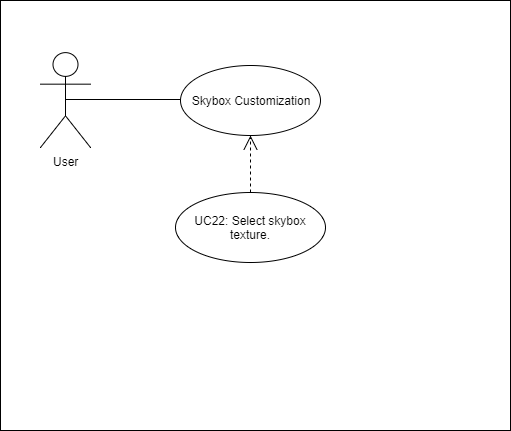
\includegraphics[width=250px,height=150px]{SkyboxCustomization.png}
	\end{center}

	\textbf{Precondition:} The user is inside an environment with a skybox.

	\textbf{Postcondition:} The skybox texture is changed.

	\begin{itemize}
		\item Video Recording:
	\end{itemize}

	\begin{center}
	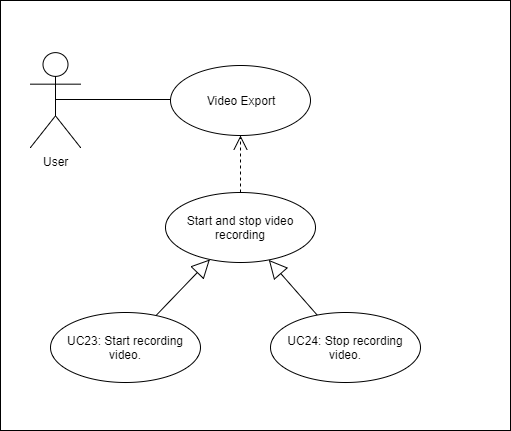
\includegraphics[width=250px,height=150px]{VideoExport.png}
	\end{center}

	\textbf{Precondition:} The user is inside an environment.

	\textbf{Postcondition:} A 360 degree video is recorded and saved within the asset folder.
	\end{flushleft}

\subsection{Target Audience Characteristics}

	Initially we planned on focusing our attention on optimizing the presentation software for the education sector, and then extending it to include the corporate world by optimizing a different profile for a business setting.  However we later realised that to broaden our target audience, we could design the presentation software to be community driven in terms of content.  This would allow virtually anyone to use the software, as well as contribute to an ever-growing community-driven collection of materials, which, of corse, they would also have at their complete disposal.

\subsection{Constraints}
There are several constraints needed to be taken into consideration.
\bigskip
\begin{flushleft}
\textsl{Platform constraints:}
\end{flushleft}
	\begin{itemize}
		\item Mono, an open source development platform based on the .NET Framework. Mono’s implementation is based on the ECMA standards for C\# and the Common Language Infrastructure.
		\item For development:
			\begin{itemize}
				\item Windows 7 SP1+, 8, 10; Mac OS X 10.8+.
			\end{itemize}
		\item For running Unity applications/games (depending on the complexity of the project):
			\begin{itemize}
				\item Windows XP SP2+, Mac OS X 10.8+, Ubuntu 12.04+, SteamOS+.
			\end{itemize}
	\end{itemize}
\medskip
\textsl{Device hardware constraints:}
	\begin{itemize}
		\item Graphics card: DX9 (shader model 3.0) or DX11 with feature level 9.3 capabilities.
		\item CPU: SSE2 instruction set support.
	\end{itemize}
\medskip
\textsl{Video size:}
	\begin{itemize}
		\item The exported video should be a realistic size, taking bandwidth and cap into consideration.
	\end{itemize}
\medskip
\textsl{Community content needs to be a reasonable size (in community guidelines):}
	\begin{itemize}
		\item Contributing to the complexity of a project will increase exported video size.
	\end{itemize}
\medskip
\textsl{Community content needs to be relatively optimized (in community guidelines):}
	\begin{itemize}
		\item Again, contributing to the complexity of a project will increase exported video size.
	\end{itemize}
\medskip
\textsl{Other constraints that will be considered and in which further research will be conducted as implementation progresses include:}
	\begin{itemize}
		\item Possible VR device constraints with regards to environment editing.
		\item Fixed set of templates.
		\item Unity assets only for community driven content.
	\end{itemize}

\newpage

\subsection{Testing Framework}
	\subsubsection{Introduction}
		The 3D VR Presentations project presents a unique problem when it comes to testing.\\
		Because the primary goals of the project is to create an intuitive and easy to use interface to create presentations,
		the assessment will be qualitative in nature.\\
		Thus traditional methods of testing such as unit tests and e2e tests will not be useful to determine if we are creating a viable and working product.\\
		However some parts should still be able to be tested in that way. Further research is needed in order to determine a way of implementing unit and e2e tests and which framework will be used for them.\\
		We are planning on utilizing usability testing at the end of each phase in order to determine how viable our current product is at that stage.\\
		We are also looking into Agile UX Design Principles.

	\subsubsection{Usability Testing}
		In short, Usability Testing is a way to see how easy to use something is by testing it with real users.\\
		At the end of each sprint we will test our product in its current state with real users and based on their feedback we will plan adjustments to our development.
		We will be using knowledge that we have gained from IMY310 to that end.

	\subsubsection{Agile UX Principles}
		I have absolutely no idea what to say here. I can't find concensus on any online sources except for what I have already described above.\\
		Could whomever reviews this please assist?

\subsection{Technologies}
	\subsubsection{Initial Technologies}
		In our first meeting with EPI-USE we had discussed the use of various technologies. They had given us "free will" with regards to what technologies to use. We are considering the following technolgies:
		\begin{itemize}
			\item Creating a 3D environment to design and bring to life a 3D presentation.
			\item Unity 3D virtual reality system tool kit library.
			\item HTC Vive virtual reality gear (already available).
			\item Import external models.
			\item Using plug and play libraries.
			\item Possibly include library templates for uses to build on.
			\item Community driven approach.
			\item Windows 10 environment.
		\end{itemize}

	\subsubsection{Technologies to be used}
		After looking into the above technologies as well as other technologies that are not listed, we have narrowed our choices down to the following:
		\begin{itemize}
			\item Unity Game Engine \\
			We decided to utitlize the Unity Game Engine because of the massive amount of documentation and support that it has. We also received a lot of recommendations from people who work in the industry to use Unity.\\

			\item Unity open-source plugins \\
			Unity has a lot of community-created plugins that might be useful with our project. Which plugins will be used will be determined as we delve deeper into the project. \\

			\item Unity VR library \\
			Unity has support for both the Oculus Rift and the HTC Vive. This will help should we run into issues with the specific hardware. \\

			\item Visual Studio \\
			We will be using Visual Studio in order to create the interface as it is quite easy to use, and because Unity comes bundled with it. \\

			\item Github \\
			We already have a repository on Github that we are using to collaborate on the project. Github is very user friendly and has a lot of tools that make project management easier.
		\end{itemize}

\newpage

  \section{Architectural Design patterns}
    During the process of creating a 3D environment we have employed the effectiveness of certain design patterns to help simplify the interaction between the user and the environment itself. The architectural patterns we have used are as follows:\\\\
    1.	Factory Design Pattern\\
    2.	Memento Design Pattern\\
    3.	Prototype Design Pattern\\
  	\subsection{Justification of Design pattern use:}
  	\subsubsection{Factory}
  	In the VR presentation software we have created an interface whereby the players/users are able to create and instantiate 3D objects. This creation is facilitated through our use of a factory design method. By providing the interface for the user to create these 3D objects they can then make use of a set of subclasses to determine the specifics of what objects is to be made.\\
  	\subsubsection{Memento}
  	We plan to utilize the memento design pattern in a manner that is seen across many different gaming environments. Due to users being able to create customized worlds and environments it became an imperative that they are able to save their work. The ability to capture the game environments internal state and then recall that from storage will be executed with the Memento design pattern to allow restoration to a specific point.\\
  	\subsubsection{Prototype}
  	In the 3D environment one of the essential functions was that after a user had finished scaling and rotation an object they should be able to create a duplicate of this object, using the pre-existing object as some form of prototype. This meant that through implementing the Prototype design pattern we were able to create a platform where they could achieve this cloning functionality.
    \subsection{Actvity Diagram}
  	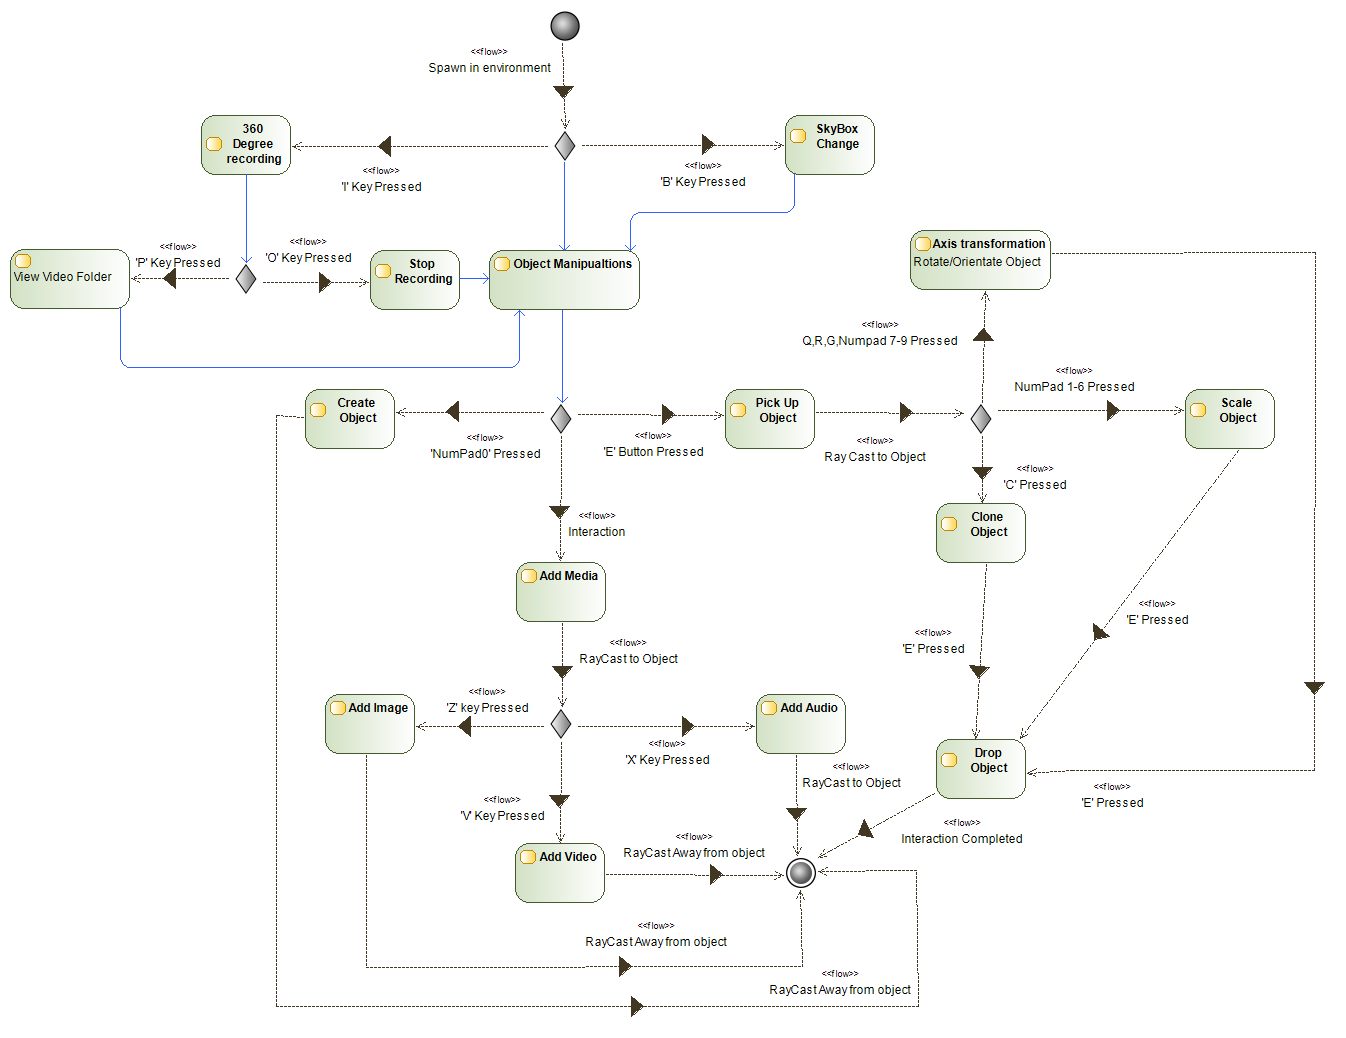
\includegraphics[width=450px,height=325px]{ActivityDiagram.png}

  	\subsection{Deployment Diagram:}
  	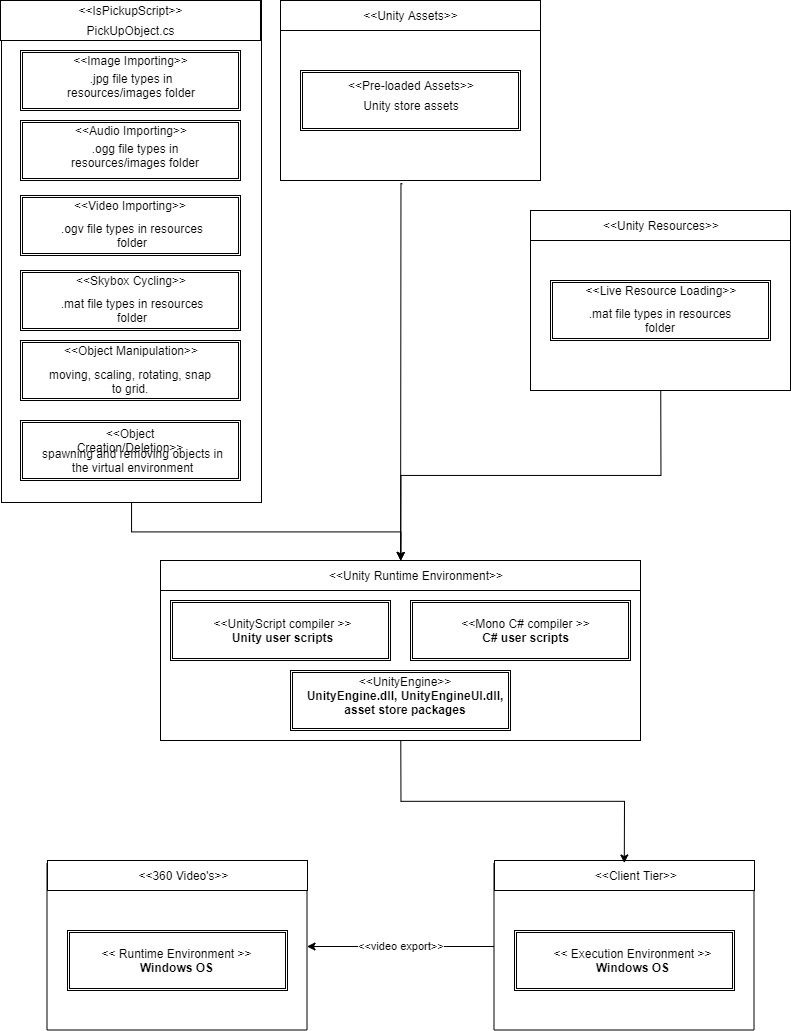
\includegraphics[width=450px,height=550px]{DeploymentDiagram.png}



\end{document}
